\section{Phân tích chi tiết bài báo}
\subsection{Giới thiệu}
Các cuộc tấn công nâng cao và liên tục (APTs) ngày càng tinh vi được thực hiện bởi những kẻ tấn công có kỹ năng cao, gây ra mối đe dọa lớn cho cả các doanh nghiệp và tổ chức. Hiện nay, có nhiều phương pháp phát hiện APT dựa trên phân tích đồ thị nguồn gốc dữ liệu, nhằm trích xuất thông tin từ các bản ghi nhật ký và hỗ trợ phát hiện các mối đe dọa. Tuy nhiên, các phương pháp hiện tại vẫn còn gặp nhiều thách thức. Thiếu dữ liệu (LOD) trong các phương pháp có giám sát, yêu cầu kiến thức tiên nghiệm về APT, làm chúng dễ bị tấn công bởi các mối đe dọa mới. Tỷ lệ dương tính giả cao ở các phương pháp dựa trên thống kê, do không thể trích xuất ngữ nghĩa sâu từ các bản ghi. Chi phí tính toán lớn của các phương pháp học sâu, đặc biệt là các phương pháp dựa trên chuỗi và đồ thị, gây khó khăn trong việc triển khai thực tế.

Để giải quyết những vấn đề này, bài báo giới thiệu MAGIC, một phương pháp phát hiện APT tự giám sát mới. MAGIC kết hợp học biểu diễn đồ thị có che với các phương pháp phát hiện ngoại lệ đơn giản. MAGIC trước tiên xây dựng đồ thị từ các bản ghi nhật ký và sau đó sử dụng mô-đun auto-encoder đồ thị có che để tạo biểu diễn nhúng. Các biểu diễn này được phân tích bằng phương pháp phát hiện ngoại lệ không giám sát, giúp nhận diện các thực thể hệ thống bị tấn công.
MAGIC được thiết kế với tính linh hoạt cao, cho phép phát hiện ở nhiều cấp độ khác nhau, từ phát hiện APT theo lô đến xác định đối tượng tấn công cụ thể. Nó có thể hoạt động hiệu quả trong cả môi trường không giám sát, bán giám sát, và giám sát hoàn toàn. Ngoài ra, MAGIC còn bao gồm một cơ chế thích nghi mô hình, giúp giảm tỷ lệ dương tính giả thông qua phản hồi từ người dùng
MAGIC đã được đánh giá trên ba bộ dữ liệu APT khác nhau (DARPA Transparent Computing E3, StreamSpot, và Unicorn Wget), với các kết quả ấn tượng: độ chính xác 97,26\%, độ nhạy 99,91\%, và hiệu suất tính toán vượt trội so với các phương pháp hiện có, nhanh hơn ShadeWatcher tới 51 lần.

\subsection{Phương Pháp}

\subsubsection{Tổng quan về MAGIC}
MAGIC (Masked Graph Representation Learning for APT Detection) là một phương pháp học máy tự giám sát kết hợp với phát hiện ngoại lệ trên đồ thị nhằm mục đích phát hiện các mối đe dọa liên tục nâng cao (APTs). Các thành phần chính trong phương pháp của hệ thống này:
\begin{itemize}
    \item \textbf{Xây dựng biểu đồ nguồn gốc (Provenance Graph Construction).}
    \item \textbf{Mô-đun học biểu diễn đồ thị (Graph Representation Module).}
    \item \textbf{Mô-đun phát hiện (Detection Module).}
    \item \textbf{Cơ chế thích nghi mô hình (Model Adaption Mechanism).}
\end{itemize}
\begin{figure}
    \centering
    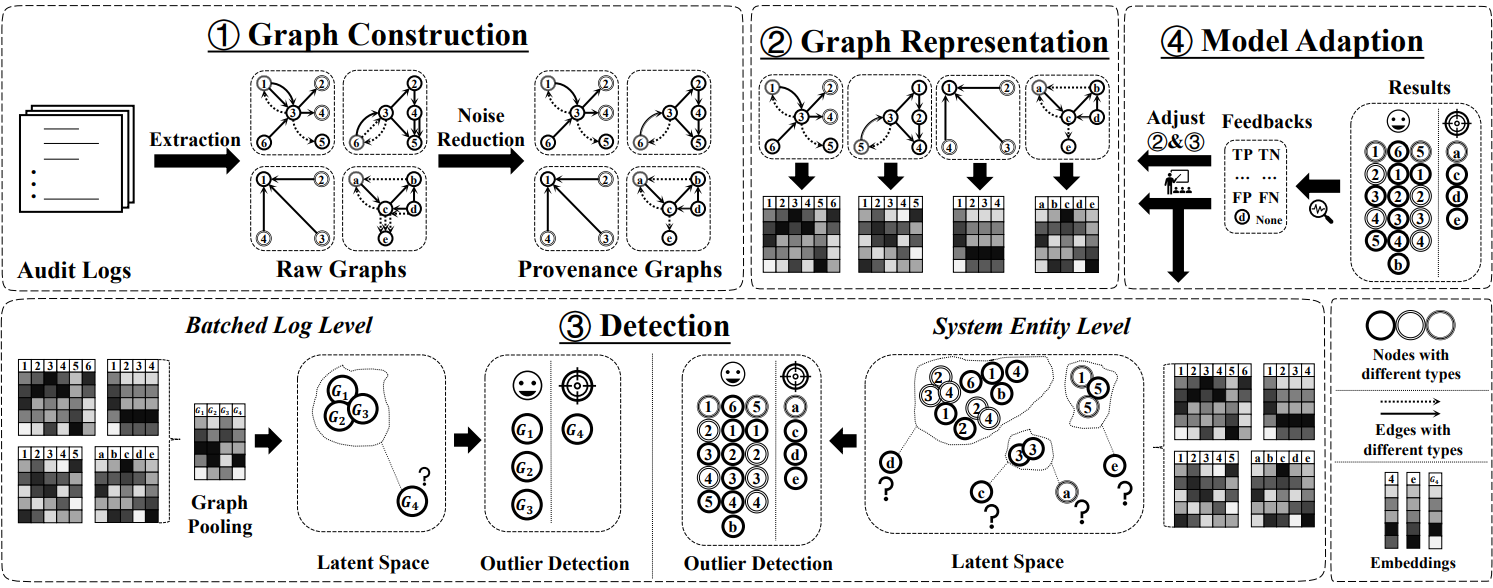
\includegraphics[width=1\linewidth]{Overview_of_MAGIC_s_detection_pipeline.png}
    \caption{Tổng qua về pipeline phát hiện bất thường của MAGIC}
    \label{fig:Overview_of_MAGIC_s_detection_pipeline}
\end{figure}
\subsubsection{Xây dựng biểu đồ nguồn gốc (Provenance Graph Construction)}
Biểu đồ nguồn gốc được xây dựng từ các nhật ký kiểm toán hệ thống. Các nút và cạnh là các thực thể hệ thống và các tương tác trong các nhật ký:

\begin{itemize}
    \item \textbf{Log Parsing:} Phân tích từng mục nhật ký để trích xuất các thực thể hệ thống (ví dụ: các tiến trình, tệp tin, luồng mạng,...) tương ứng là các nút và các tương tác giữa chúng (ví dụ: thực thi, đọc, kết nối,...) tương ứng là các cạnh của đồ thị.
    \item \textbf{Embedding ban đầu:} Gán các nhãn cho các nút và cạnh để biến chúng thành các vector đặc trưng.
    \item \textbf{Giảm nhiễu (Noise Reduction):} Để làm giảm độ phức tạp, MAGIC kết hợp các cạnh dư thừa giữa các cặp nút để tạo ra một cạnh duy nhất.
\end{itemize}
\begin{figure}[!h] %
    \centering
    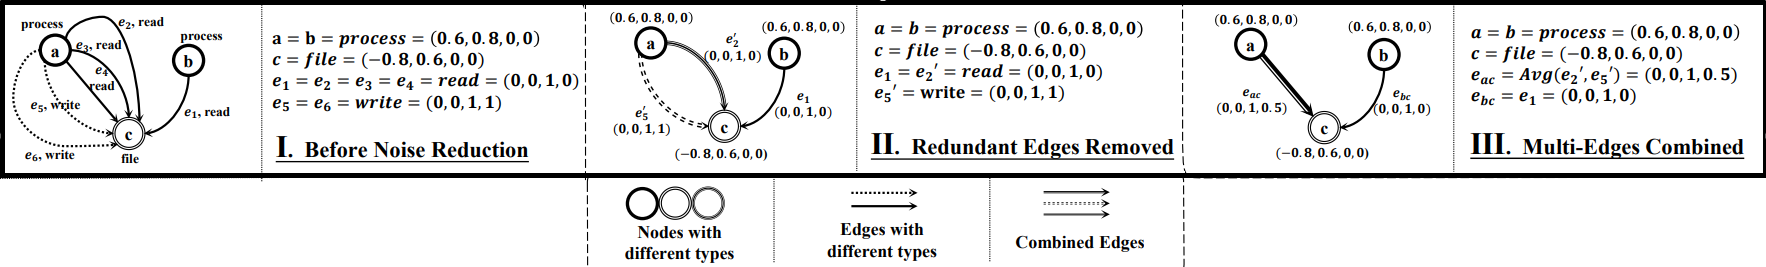
\includegraphics[width=1\linewidth]{Example_of_MAGIC_s_graph_construction_steps_1.png}
    \caption{Ví dụ các bước tạo đồ thị của mô hình MAGIC}
    \label{fig:enter-label}
\end{figure}
\subsubsection{Mô-đun học biểu diễn đồ thị (Graph Representation Module)}
Mô-đun học biểu diễn đồ thị của MAGIC nhằm tạo ra các vector biểu diễn hiệu quả cho các thực thể và trạng thái hệ thống:

\begin{itemize}
    \item \textbf{Masked Graph Auto-Encoders:} Sử dụng bộ Auto-Encoders để học tự giám sát các biểu diễn :
    \begin{itemize}
        \item \textbf{Feature Masking:} Các nút trong đồ thị sẽ được che ngẫu nhiên trong quá trình huấn luyện để mô hình học được các đặc trưng ẩn sâu trong biểu đồ mà không cần nhãn.
        \item \textbf{Graph Encoder:} MAGIC sử dụng mạng attention trên đồ thị (GAT) để lan truyền và tổng hợp các đặc trưng từ các nút láng giềng. 
        \item \textbf{Graph Decoder:} Khôi phục lại các nút đã bị che để tối ưu hóa biểu diễn đồ thị. 
    \end{itemize}
    \item \textbf{Pooling and Embeddings:}
    \begin{itemize}
        \item Sau khi đi qua các lớp GAT, MAGIC kết hợp các vector biểu diễn từ các nút để tạo ra một biểu diễn tổng thể của trạng thái hệ thống. 
    \end{itemize}
\end{itemize}

\subsubsection{Mô-đun phát hiện ngoại lệ (Detection Module)}
Dựa trên các biểu diễn đã học, MAGIC sử dụng mô-đun phát hiện ngoại lệ để phát hiện các thực thể hoặc trạng thái của hệ thống là bất thường:

\begin{itemize}
    \item \textbf{Outlier Detection:} Khi có một thực thể mới, MAGIC tìm kiếm các láng giềng gần nhất của nó trong cây K-D và tính toán độ giống nhau (similarity) giữa chúng.
    \item \textbf{Anomaly Scoring:} MAGIC sử dụng khoảng cách Euclidean để đánh giá điểm ngoại lệ của một thực thể. Nếu điểm này vượt quá ngưỡng định trước, thực thể đó được đánh dấu là độc hại.
    \item \textbf{Batched Log Level Detection:} MAGIC sẽ cảnh báo nếu phát hiện thấy các trạng thái bất thường của lô nhật ký.
    \item \textbf{System Entity Level Detection:} Phát hiện các thực thể có hành vi bất thường.
\end{itemize}

\subsubsection{Cơ chế thích nghi mô hình (Model Adaption Mechanism)}
MAGIC có cơ chế thích nghi để đối phó với sự thay đổi của hệ thống (concept drift):

\begin{itemize}
    \item \textbf{Feedback Learning:} Các kết quả phát hiện được xác nhận bởi người dùng sẽ được đưa lại vào MAGIC. Mô hình có thể học từ những hành vi hệ thống mới này và cải thiện khả năng phát hiện.
    \item \textbf{Memory Management:} Khi dữ liệu học từ feedbacks ngày càng nhiều, MAGIC sẽ loại bỏ các dữ liệu cũ để duy trì hiệu suất và giảm thiểu việc cảnh báo sai (false positives). Thông qua đó, MAGIC có thể thích nghi với các thay đổi hệ thống mới mà không bị giảm hiệu quả.
\end{itemize}

\subsection{Thực nghiệm và đánh giá của tác giả}
Hình \ref{fig:datasets} giới thiệu ba bộ dữ liệu được sử dụng để đánh giá MAGIC. Dataset StreamSpot là một tập nhỏ gồm 600 lô nhật ký hệ thống, trong đó có một kịch bản tấn công. Dataset Unicorn Wget chứa 150 lô, trong đó có 25 lô với các cuộc tấn công chuỗi cung ứng khó phát hiện. Dataset DARPA E3, với hơn 51GB dữ liệu và hàng triệu thực thể hệ thống, đánh giá khả năng phát hiện của MAGIC trong môi trường phức tạp và quy mô lớn.
\begin{figure}
    \centering
    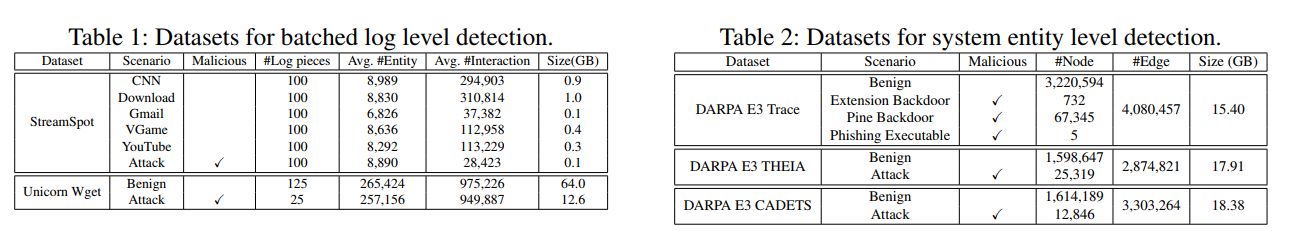
\includegraphics[width=1\linewidth]{datasets.png}
    \caption{Các dataset thực nghiệm}
    \label{fig:datasets}
\end{figure}

Kết quả cho thấy MAGIC phát hiện APT với độ chính xác cao trong nhiều kịch bản khác nhau như \ref{fig:results_on_various_dataset}

\begin{figure}
    \centering
    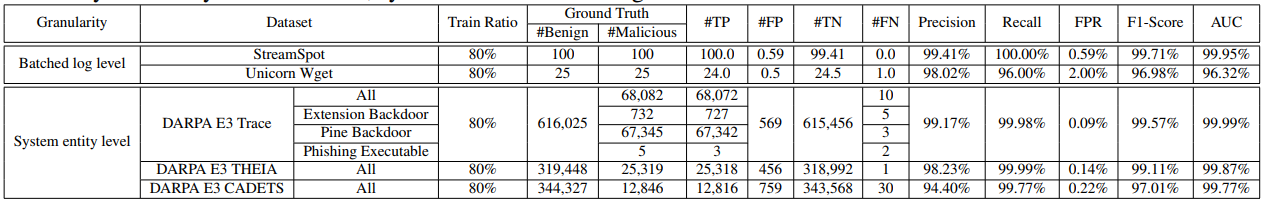
\includegraphics[width=0.5\linewidth]{results_on_various_dataset.png}
    \caption{Kết quả phát hiện của MAGIC trên các bộ dữ liệu khác nhau}
    \label{fig:results_on_various_dataset}
\end{figure}

\begin{figure}
    \centering
    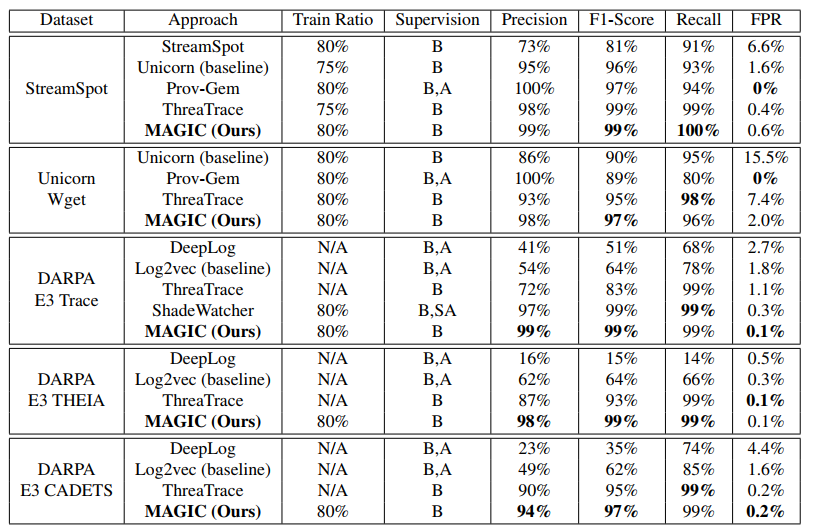
\includegraphics[width=0.5\linewidth]{compare_various_dataset.png}
    \caption{So sánh giữa MAGIC và các phương pháp phát hiện APT hiện đại trên các bộ dữ liệu khác nhau}
    \label{fig:compare_various_dataset}
\end{figure}

MAGIC cho thấy hiệu quả cao trong việc phát hiện APT trên ba bộ dữ liệu khác nhau như hình \ref{fig:compare_various_dataset}. Cụ thể:

Bộ dữ liệu StreamSpot: MAGIC đạt gần như kết quả hoàn hảo. MAGIC đạt độ chính xác trung bình 98.01\% và độ hồi đáp 96.00\%.

% Bộ dữ liệu StreamSpot: MAGIC đạt gần như kết quả hoàn hảo do chỉ có một hoạt động người dùng trong mỗi lô nhật ký, giúp tách biệt dễ dàng hành vi hệ thống. MAGIC đạt độ chính xác trung bình 98.01\% và độ hồi đáp 96.00\%.

Bộ dữ liệu Unicorn Wget: Mặc dù khó phân biệt các cuộc tấn công ẩn nấp với hành vi lành tính, MAGIC vẫn phát hiện được 24/25 lô nhật ký tấn công với 0.5 dương tính giả.

Bộ dữ liệu DARPA E3: MAGIC đạt 99.91\% độ hồi đáp và tỷ lệ dương tính giả 0.15\%. 
% Nó dễ dàng phát hiện các quy trình và kết nối độc hại, nhưng gặp khó khăn với các tệp và thư viện độc hại do chúng có hành vi tương tự như các thực thể lành tính.

Kết quả cho thấy MAGIC vượt trội so với các phương pháp phát hiện APT hiện đại khác, như Unicorn, Prov-Gem, và ThreaTrace, về độ chính xác và hiệu suất.

MAGIC hoạt động với mức tiêu tốn tài nguyên tối thiểu, nhanh hơn nhiều lần so với các phương pháp tiên tiến nhất, giúp nó có thể áp dụng trong nhiều điều kiện khác nhau \ref{fig:magic_results_cost}.
\begin{figure}
    \centering
    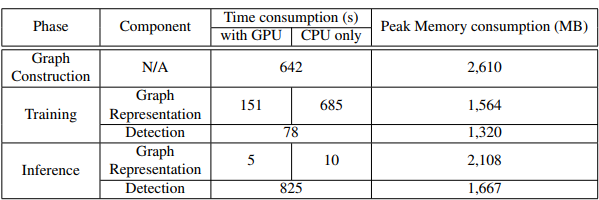
\includegraphics[width=0.5\linewidth]{magic_results_cost.png}
    \caption{Chi phí hiệu suất của MAGIC trên tập dữ liệu con E3-Trace}
    \label{fig:magic_results_cost}
\end{figure}

Bảng \ref{fig:false_positive} trình bày kết quả thử nghiệm của MAGIC trên tập dữ liệu Trace, đặc biệt là hiệu quả của cơ chế điều chỉnh mô hình trong việc giảm số lượng false positives trong các bản ghi audit hợp lệ.

\begin{figure}
    \centering
    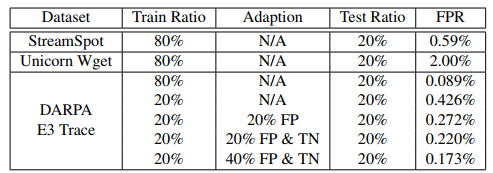
\includegraphics[width=0.5\linewidth]{false_positive.png}
    \caption{Tỷ lệ dương tính giả của MAGIC trên các tập dữ liệu khác nhau}
    \label{fig:false_positive}
\end{figure}
\subsection{Kết luận của tác giả}

MAGIC là một phương pháp phát hiện APT không cần giám sát, dựa trên mô hình hóa hành vi và phát hiện điểm bất thường. Áp dụng rộng rãi với chi phí tính toán thấp. Nó sử dụng học biểu diễn đồ thị để mô hình hóa hành vi hệ thống lành tính từ các nhật ký kiểm tra và phát hiện APT thông qua các phương pháp phát hiện ngoại lệ. Đánh giá trên ba bộ dữ liệu cho thấy MAGIC đạt kết quả tốt với tỷ lệ dương tính giả thấp và chi phí tính toán tối thiểu.